% LQR position controller with DARE-computed state-feedback gain.
% Compile: pdflatex position-loop-lqr.tex && pdf2svg ...
\documentclass[tikz, margin=4mm]{standalone}
\usetikzlibrary{arrows.meta, positioning, calc}

\tikzset{
  block/.style = {draw, rectangle, rounded corners=2pt, align=center,
                  fill=blue!8, font=\small,
                  minimum height=1.0cm, minimum width=2.8cm},
  sum/.style   = {draw, circle, fill=blue!8, minimum size=7mm, inner sep=0pt},
  arr/.style   = {-{Latex[length=4pt, width=5pt]}, thick},
  lbl/.style   = {font=\footnotesize},
  node distance = 0.9cm and 1.8cm
}

\begin{document}
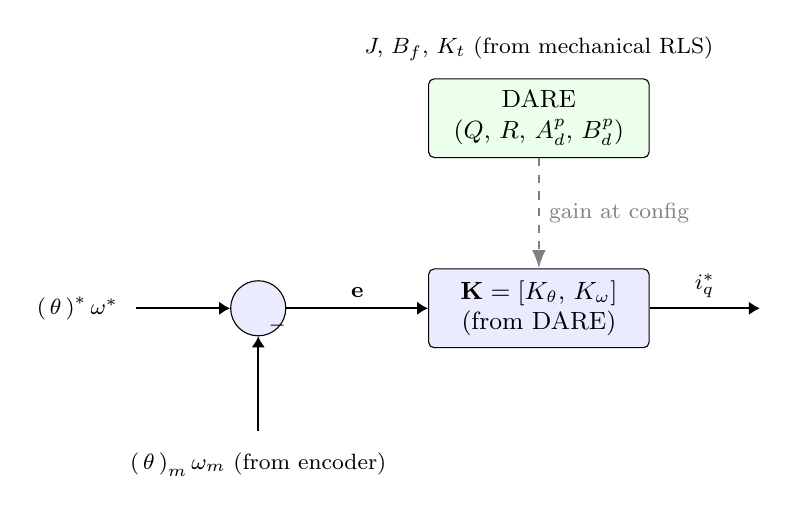
\begin{tikzpicture}

  % ── Reference error ───────────────────────────────────────────────────────
  \node[sum]                           (Se)   {};    % error: x* − x
  \node[block, right=1.8cm of Se]      (Kgain) {$\mathbf{K} = [K_\theta,\,K_\omega]$\\ (from DARE)};

  % ── Output ───────────────────────────────────────────────────────────────
  \coordinate (IqOut) at ($(Kgain.east)+(1.4,0)$);

  % ── State references ─────────────────────────────────────────────────────
  \coordinate (XrefIn) at ($(Se.west)+(-1.2,0)$);
  % State measurement feedback
  \coordinate (XmIn)   at ($(Se.south)+(0,-1.2)$);

  % ── DARE configuration (offline) ─────────────────────────────────────────
  \node[block, above=1.4cm of Kgain, fill=green!8]
        (DARE) {DARE\\ ($Q$, $R$, $A_d^p$, $B_d^p$)};

  % ── Connections ───────────────────────────────────────────────────────────

  % Reference input
  \node[lbl, left=0.1cm of XrefIn] {$\begin{pmatrix}\theta^*\\\omega^*\end{pmatrix}$};
  \draw[arr] (XrefIn) -- (Se);

  % Error → gain → iq*
  \draw[arr] (Se)      -- node[lbl,above]{$\mathbf{e}$} (Kgain);
  \draw[arr] (Kgain.east) -- node[lbl,above]{$i_q^*$}   (IqOut);

  % State feedback (negative)
  \node[lbl, below=0.15cm of XmIn]
        {$\begin{pmatrix}\theta_m\\\omega_m\end{pmatrix}$ (from encoder)};
  \draw[arr] (XmIn) -- (XmIn -| Se) -- (Se)
             node[below right, font=\scriptsize]{$-$};

  % DARE → gain (configuration time only, shown dashed)
  \draw[dashed, -Latex, thick, gray]
       (DARE.south) -- node[lbl, right]{gain at config} (Kgain.north);

  % RLS parameters to DARE
  \node[lbl, above=0.1cm of DARE] {$J,\,B_f,\,K_t$ (from mechanical RLS)};

\end{tikzpicture}
\end{document}
